\newcommand{\doctitle}{计算机系统结构第二次作业}
\documentclass[oneside,a4paper]{article}

\usepackage{parskip}
\usepackage{subfigure}
% \usepackage{geometry}
\usepackage{amsmath}
\usepackage[dvipdfm]{graphicx} 
\usepackage{amsthm,amssymb}
\usepackage{tikz}
\usepackage{fontspec,xltxtra,xunicode}


\usepackage{fancyvrb}
% \usepackage{fancybox}
\usepackage{listings}
\lstset{numbers=left, 
  numberstyle=\scriptsize,
  frame=single,
  flexiblecolumns=false,
  language=,
  texcl=true,
  escapechar=\%,
  basicstyle=\ttfamily\small, 
  breaklines=true,
  extendedchars=true,
  showstringspaces=false,
  keywordstyle=\bfseries}

% \usepackage{indentfirst} 


\usepackage{pstricks} 
\usepackage[dvipdfm,a4paper,
hyperindex=true,
backref=section,
bookmarks=true,
bookmarksnumbered=true,
pdfpagemode=UseOutlines,
pdffitwindow=true,
linkbordercolor=white, % 链接边框设置为白色
citebordercolor=white, % 链接边框设置为白色
urlbordercolor=white]{hyperref}
          

% \DefineShortVerb{\|}

\usepackage{xeCJK}
\setCJKmainfont[BoldFont={Adobe Heiti Std}, ItalicFont={Adobe Kaiti Std}]{Adobe Song Std}
\setCJKmonofont{Adobe Fangsong Std}
\xeCJKsetcharclass{"0}{"2E7F}{0}
\xeCJKsetcharclass{"2E80}{"FFFF}{1}

\setmainfont[Mapping=tex-text]{Linux Libertine O}
\setsansfont[Mapping=tex-text]{Linux Biolinum O} 
\setmonofont{Courier 10 Pitch} 
\punctstyle{quanjiao} 


\renewcommand{\figurename}{图}
\renewcommand{\tablename}{表}
\renewcommand{\lstlistingname}{程序清单}

\newenvironment{solve}{%
  \settowidth{\leftskip}{\textit{解:}\ }%
  \makebox[0pt][r]{\textit{解:}\ }%
  \ignorespaces}{\qed\par\ignorespacesafterend}

\author{\textsc{Computer Science} 0813\\谢松 U200814454}
\title{\doctitle}
\hypersetup{
  pdftitle={\doctitle},
  pdfauthor={谢松},
  pdfsubject={\doctitle}}
\usepackage{booktabs}

\begin{document}


\maketitle

%%% Local Variables: 
%%% mode: latex
%%% TeX-master: t
%%% End: 


\section{Ex 3.8}

\begin{solve}
  对于$\sum_{i=1}^4{A_i\times{}B_i}$, 应首先计算$A_i\times{}B_i$, 然后
  计算$A_1\times{}B_1 + A_2\times{}B_2$和$A_3\times{}B_3 +
  A_4\times{}B_4$, 最后计算$A_1\times{}B_1 + A_2\times{}B_2 +
  A_3\times{}B_3 + A_4\times{}B_4$.

  绘出该计算的流水线时空图, 如图~\ref{fig:pipe1}所示, 其中阴影部分表示
  相应的功能段在工作, 标有蓝色阴影的步骤表示乘法, 标有红色阴影的步骤表
  示加法.

  \begin{figure}[!h]
    \centering
    \begin{tikzpicture}[scale=0.5, mul/.style = {rectangle, draw=blue,
        thick, fill=blue!20, minimum size = 0.5cm, text centered},
      add/.style = {rectangle, draw=red, thick, fill=red!20, minimum
        size = 0.5cm, text centered}]
      \draw[step=1, help lines](0, 0) grid (18, 5);
      \begin{scope}
        \draw[->] (0, 0) -- (19, 0) node[below] {时间} coordinate(x
        axis); \draw[->] (0, 0) -- (0, 6) node[left] {部件}
        coordinate(y axis); \foreach \x in {1, ..., 18}
        \draw[xshift=\x cm - 0.5cm] node[below] {\x}; \foreach \y in
        {1, ..., 5} \draw[yshift=\y cm - 0.5cm] node[left] {\y};
      \end{scope}
      \draw +(0.5cm, 0.5) node[mul] {1} +(1 cm * 2, 1.5) node[mul,
      minimum width = 1cm] {1} +(1 cm * 2 + 1.5 cm, 4.5) node[mul]
      {1}; \foreach \s in {2, ..., 4} \draw +(2 * \s cm - 2.5cm, 0.5)
      node[mul] {\s} +(\s cm * 2, 1.5) node[mul, minimum width = 1cm]
      {\s} +(\s cm * 2 + 1.5 cm, 4.5) node[mul] {\s};
      \foreach \t in {1, 2} {
        \draw +(4.5cm + 3*\t cm, 0.5 cm) node[add] {\t};
        \foreach \s in {3, 4, 5}
        \draw +(2.5cm + 3 * \t cm + \s cm, \s cm - 0.5 cm) node[add] {\t};
      }
      \draw +(14.5cm, 0.5cm) node[add] {3};
      \foreach \s in {3, 4, 5}
      \draw +(12.5cm + \s cm, \s cm - 0.5 cm) node[add] {3};
    \end{tikzpicture}
    \label{fig:pipe1}
    \caption{流水线时空图}
  \end{figure}
  
  由图~\ref{fig:pipe1}可见, 流水线在18个$\Delta{}t$的时间内, 给出了7个
  结果, 故吞吐率$TP$为:
  \begin{displaymath}
    TP = \frac{7}{18\Delta{}t}.
  \end{displaymath}

  若不使用流水线, 求一次积或和均需要$4\Delta{}t$的时间, 那么产生上述7个
  结果需要$4\times{}7\Delta{}t = 28\Delta{}t$的时间. 故加速比$S$为:
  \begin{displaymath}
    S = \frac{28\Delta{}t}{18\Delta{}t} \approx 1.56
  \end{displaymath}

  流水线的效率可以有阴影部分面积和与5个功能段时空区的面积的比值, 求得效
  率$E$为:
  \begin{displaymath}
    E = \frac{4\times{}7}{5\times{}18} \approx 0.31
  \end{displaymath}
\end{solve}

\section{Ex 3.10}

\begin{solve}
  根据预约表写出禁止表$F = \{1, 3, 6\}$. 从而得到冲突向量$C_0 =
  (100101)$.
  
  使用如程序清单~\ref{lst:3-10}所示的C++程序, 输出求得的状态转移图
  的Graphviz代码, 根据Graphviz绘得的图, 重新排版得到如图~\ref{fig:3-10}所
  示的状态转移图.

  \begin{figure}[!h]
    \centering
    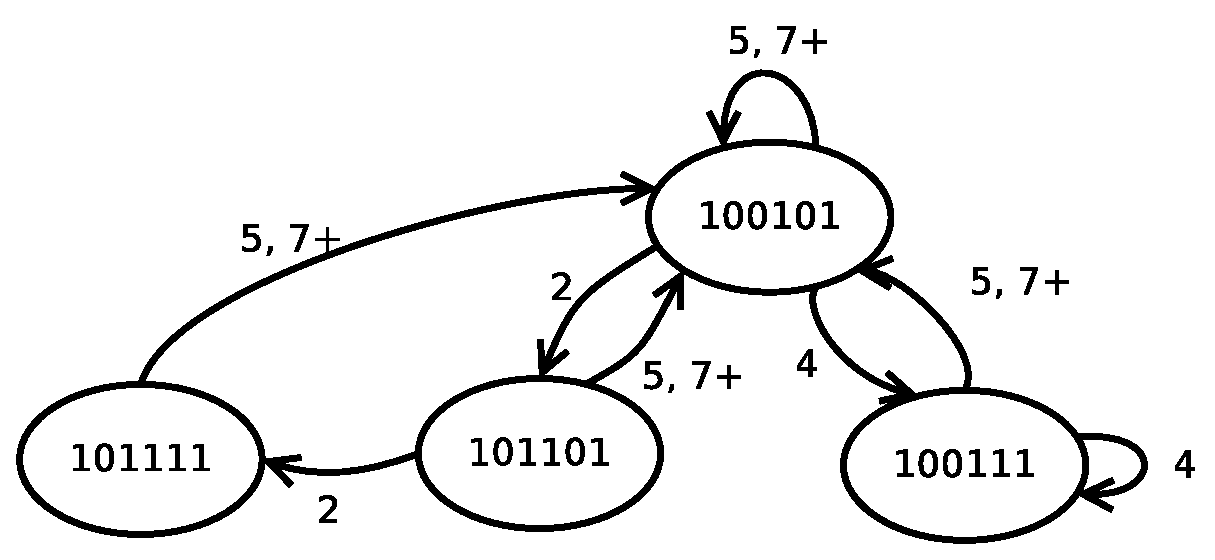
\includegraphics[width=0.6\textwidth]{img/3-10.eps}
    \caption{状态转移图}
    \label{fig:3-10}
  \end{figure}
  
  \lstinputlisting[language=C++, caption=绘制状态转移图的C++代码, label=lst:3-10]{3-10.cpp}

  根据状态转移图, 得到可能的调度策略及平均延迟拍数如表~\ref{tab:3-10}
  所示.

  \begin{table}[!h]
    \centering
    \begin{tabular}{cc}
      \toprule
      调度策略 & 平均延迟拍数 \\ \midrule
      (2, 2, 5) & 3 \\
      (2, 5) & 3.5 \\
      (4, 5) & 4.5 \\
      (4) & 4 \\
      (5) & 5 \\ \bottomrule
      
    \end{tabular}
    \caption{可能的调度策略及平均延迟拍数}
    \label{tab:3-10}
  \end{table}

  根据表~\ref{tab:3-10}中的数据可知, 最优等间隔调度策略是(4), 它的最
  大吞吐率为
  
  \begin{align*}
    TP_{1_{\mathrm{max}}} &=
    \lim_{n\rightarrow{}\infty}{\frac{n}{7+4(n-1)\Delta{}t}}\\
    &=\frac{1}{4\Delta{}t};
  \end{align*}

  最优不等间隔调度策略是(2, 2, 5), 它的最大吞吐率为

  \begin{align*}
    TP_{2_{\mathrm{max}}} &=
    \lim_{n\rightarrow{}\infty}{\frac{n}{7+3(n-1)\Delta{}t}}\\
    &=\frac{1}{3\Delta{}t}.
  \end{align*}

  若输入10个任务, 那么最优等间隔调度的实际吞吐率为
  
  \begin{align*}
    TP_1 &= \frac{10}{7+4\times{}9 \Delta{}t}\\
    &= \frac{10}{43\Delta{}t},
  \end{align*}

  加速比为

  \begin{align*}
    S_1 &= \frac{10\times{}7}{7+(10-1) \times{} 4}\\
    &= \frac{70}{43} \approx 1.63;
  \end{align*}

  最优不等间隔调度的实际吞吐率为
  
  \begin{align*}
    TP_2 &= \frac{10}{(7+2+2+5+2+2+5+2+2+5)\Delta{}t}\\
    &= \frac{10}{34\Delta{}t} 
  \end{align*}

  加速比为

  \begin{align*}
    S_2 &= \frac{10\times{}7}{7+2+2+5+2+2+5+2+2+5}\\
    &= \frac{35}{17} \approx 2.06
  \end{align*}
\end{solve}

\section{Ex 3.11}

\begin{solve}
  \begin{enumerate}
  \item 无Forwarding, 排空流水线的情况下的时空图

    \begin{flushleft}
      \footnotesize
      \begin{tabular}{@{~}lc@{~}c@{~}c@{~}c@{~}c@{~}c@{~}c@{~}c@{~}c@{~}c@{~}c@{~}c@{~}c@{~}c@{~}c@{~}c@{~}c@{~}c@{~}c@{~}c@{~}c@{~}c@{~}c@{~}}
        指令
                        & 1  & 2  & 3  & 4  & 5  & 6  & 7  & 8  & 9  & 10 & 11 & 12 & 13 & 14 & 15 & 16 & 17 & 18 & 19 & 20 & 21 & 22 & 23 \\
        \texttt{LW}     & IF & ID & EX & M  & WB \\
        \texttt{DADDIU} &    & IF & S  & S  & ID & EX & M  & WB \\
        \texttt{SW}     &    &    &    &    & IF & S  & S  & ID & EX & M  & WB \\
        \texttt{DADDIU} &    &    &    &    &    &    &    & IF & ID & EX & M  & WB \\
        \texttt{DSUB}   &    &    &    &    &    &    &    &    & IF & S  & S  & S  & ID & EX & M  & WB \\
        \texttt{BNEZ}   &    &    &    &    &    &    &    &    &    &    &    &    & IF & S  & S  & ID & EX & M  & WB \\
        \texttt{LW}     &    &    &    &    &    &    &    &    &    &    &    &    &    &    &    & IF & S  & S  & IF & ID & EX & M  & WB \\
      \end{tabular}
    \end{flushleft}

    在这种情况下, 上述循环需要$15\times{}99 + 4 = 1489$个时钟周期.

    
  \item 正常Forwarding, 分支预测失败情况下的时空图

    \begin{flushleft}
      \footnotesize
      \begin{tabular}{@{~}lc@{~}c@{~}c@{~}c@{~}c@{~}c@{~}c@{~}c@{~}c@{~}c@{~}c@{~}c@{~}c@{~}c@{~}}
        指令
                        & 1  & 2  & 3  & 4  & 5  & 6  & 7  & 8  & 9  & 10 & 11 & 12 & 13 & 14 \\
        \texttt{LW}     & IF & ID & EX & M  & WB \\
        \texttt{DADDIU} &    & IF & S  & ID & EX & M  & WB \\
        \texttt{SW}     &    &    &    & IF & ID & EX & M  & WB \\
        \texttt{DADDIU} &    &    &    &    & IF & ID & EX & M  & WB \\
        \texttt{DSUB}   &    &    &    &    &    & IF & ID & EX & M  & WB \\
        \texttt{BNEZ}   &    &    &    &    &    &    & IF & S  & ID & EX & M  & WB \\
        \texttt{LW}     &    &    &    &    &    &    &    & IF & S  & IF & ID & EX & M  & WB \\
      \end{tabular}
    \end{flushleft}

    在这种情况下, 上述循环需要$9\times{}99 + 3 = 894$个时钟周期.
    
  \item 正常Forwarding, 单周期延迟分支, 调度后的代码如程序清单~\ref{lst:3-11-re}所示.

    \lstinputlisting[language=, caption=重调度后的代码, label={lst:3-11-re}]{3-11-re.s}
      
      \begin{flushleft}
        \footnotesize
        \begin{tabular}{@{~}lc@{~}c@{~}c@{~}c@{~}c@{~}c@{~}c@{~}c@{~}c@{~}c@{~}c@{~}}
          指令
                          & 1  & 2  & 3  & 4  & 5  & 6  & 7  & 8  & 9  & 10 & 11 \\
          \texttt{LW}     & IF & ID & EX & M  & WB \\
          \texttt{DADDIU} &    & IF & ID & EX & M  & WB \\
          \texttt{DSUB}   &    &    & IF & ID & EX & M  & WB \\
          \texttt{DADDIU} &    &    &    & IF & ID & EX & M  & WB \\
          \texttt{BNEZ}   &    &    &    &    & IF & ID & EX & M  & WB \\
          \texttt{SW}     &    &    &    &    &    & IF & ID & EX & M  & WB \\
          \texttt{LW}     &    &    &    &    &    &    & IF & ID & EX & M  & WB \\
        \end{tabular}
      \end{flushleft}

      在这种情况下, 上述循环需要$6\times{}99 + 4 = 598$个时钟周期.
  \end{enumerate}
\end{solve}
\section{Lab 2}

\begin{solve}
  \begin{enumerate}
  \item 模拟程序代码见程序清单~\ref{lst:3-11}.

    \lstinputlisting[caption={Ex 3.11 模拟程序清单}, label=lst:3-11]{3-11.s}
  \item 时钟周期比较结果如下所示:
    
      \begin{tabular}{lccc}
      \toprule
      时钟周期   & (1)  & (2) & (3) \\\midrule
      人工计算   & 1489 & 894 & 598 \\
      WinMIPS64 & 1492 & 897 & 601 \\\bottomrule
    \end{tabular}
    
  \item 人工计算和WinMIPS64模拟的结果有差异, 差异的原因是在模拟的过程
    中, 需要加入指令设置寄存器R2, R3的初值, 并且额外加了一
    条\texttt{halt}指令, 因此人工计算的时钟周期数比模拟的结果少3个时钟
    周期.
  \item 对3种不同条件的流水线模拟截图及分析如下:
    \begin{enumerate}
    \item 无Forwarding的流水线时空图如图~\ref{fig:3-11-1}所示. 
      
      \begin{figure}[!h]
        \centering
        \includegraphics[width=0.9\textwidth]{img/1.png}
        \caption{无Forwarding的流水线时空图}
        \label{fig:3-11-1}
      \end{figure}

      从图中可以看到在无Forwarding的情况下, RAW冲突频繁发生.
      
    \item 有Forwarding的流水线时空图如图~\ref{fig:3-11-2}所示. 
      
      \begin{figure}[!h]
        \centering
        \includegraphics[width=0.8\textwidth]{img/2.png}
        \caption{有Forwarding的流水线时空图}
        \label{fig:3-11-2}
      \end{figure}

      从图中可以看到在有Forwarding的情况下, 访存后立即使用数据带来的冲
      突依然无法解决, 必须引入一个时钟周期的Stall. 而且对于这样的用于循
      环的分支,预测失败不是好策略.
      
    \item 有Forwarding, 延迟分支的流水线时空图如图~\ref{fig:3-11-3}所
     示. 
     
      \begin{figure}[!h]
        \centering
        \includegraphics[width=0.65\textwidth]{img/3.png}
        \caption{有Forwarding, 延迟分支的流水线时空图}
        \label{fig:3-11-3}
      \end{figure}

      从图中可以看到, 经过重新调度后的代码在流水线中可以不用加入任
      何Stall而顺利执行, 这样代码的执行效率达到最高.
    \end{enumerate}
  
  \end{enumerate}
\end{solve}
\input{../footer}
%%% Local Variables: 
%%% mode: latex
%%% TeX-master: t
%%% End: 
